\documentclass{article}

\usepackage{arxiv}
\usepackage[utf8]{inputenc} % allow utf-8 input
\usepackage[T1]{fontenc}    % use 8-bit T1 fonts
\usepackage{hyperref}       % hyperlinks
\usepackage{url}            % simple URL typesetting
\usepackage{amsfonts}       % blackboard math symbols
\usepackage{nicefrac}       % compact symbols for 1/2, etc.
\usepackage{microtype}      % microtypography
\usepackage{graphicx}
\usepackage{natbib}
\usepackage{doi}
\usepackage{csvsimple}
\usepackage{graphicx}
\graphicspath{ {./images/} }
\usepackage{float}

\title{Algorithmic predominant melody extraction in symphonic music recordings}

\date{March 23, 2022}

\author{\href{https://oriolcolomefont.com}{
\includegraphics[scale=0.06]{orcid.pdf}\hspace{1mm}Oriol Colomé Font}\\
	Music Technology Group\\
	Universitat Pompeu Fabra\\
	Barcelona \\
}

\renewcommand{\shorttitle}{\textit Algorithmic predominant melody extraction in symphonic music recordings}

%%% Add PDF metadata to help others organize their library
\hypersetup{
pdftitle={Predominant melody extraction in symphonic music recordings},
pdfsubject={MIR},
pdfauthor={Oriol Colomé Font},
}

\begin{document}
\maketitle
\begin{abstract}
This study aims to evaluate the performance of current state-of-the-art melodic tracking algorithms while discussing its results from a scientific and musicological point of view. This work aims to highlight the complexity of analyzing and evaluating computational musicological tools due to the human nature of music performances, especially in classical music. Given the complexity of the task to be carried out, there is as yet no single ideal \textit{Pitch Detection Algorithm}, so a variety of them exist. We will be using \textit{Predominant Pitch Melodia Algorithm} featured in ESSENTIA.
\end{abstract}

\section{Introduction}
The music is about subtle and pleasing imperfections: this is a simple truth. From piano strings to guitar distortion, tape emulation plugins, and reverb. Imperfections give \textbf{context} to music. For example, you can get a sense of the musician playing the instrument as an individual or as an ensemble. The skill and passion brought to a live performance, and the unique reproduction of the idea represents a high-level concept difficult to deal with.

Our fascination with music as a species has long evaded scientific rigor. Somewhere between pattern recognition, social bonding, and a deep-seated yearning to analogize the human condition lies an explanation of why we love it and how we understand it. We create deep connections to the world around us through music. It gives lifeblood to thoughts that elude capture in language. Its subjective experience is indescribable.

\section{Methods/algorithms}
\subsection{ESSENTIA}
Essentia is an open-source C++ library for audio analysis and audio-based music information retrieval. It contains an extensive collection of algorithms, including audio input/output functionality, standard digital signal processing blocks, statistical characterization of data, a large variety of spectral, temporal, tonal, and high-level music descriptors, and tools for inference with deep learning models. Essentia is cross-platform and designed with a focus on optimization in terms of robustness, computational speed, and low memory usage, which makes it efficient for many industrial applications. The library includes Python and JavaScript bindings as well as various command-line tools and third-party extensions, which facilitate its use for fast prototyping and allow setting up research experiments very rapidly.
\subsection{\textit{Predominant Pitch Melodia} Algorithm}
This algorithm estimates the fundamental frequency of the predominant melody from polyphonic music signals using the MELODIA algorithm. It is specifically suited for music with a predominent melodic element, for example the singing voice melody in an accompanied singing recording. The approach is based on the creation and characterization of pitch contours, time continuous sequences of pitch candidates grouped using auditory streaming cues. It furthermore determines for each frame, if the predominant melody is present or not. To this end, \textit{PitchSalienceFunction}, \textit{PitchSalienceFunctionPeaks}, \textit{PitchContours}, and \textit{PitchContoursMelody} algorithms are employed.

\section{Tests}
\subsection{Dataset: \textit{Orchset}}
\textit{Orchset} is intended to be used as a dataset for the development and evaluation of melody extraction algorithms. This dataset consists of 64 audio excerpts (wav format, stereo and mono, sampled at 44.1kHz) from symphonies and symphonic poems, ballets suites and other musical forms interpreted by symphonic orchestras, mostly from the romantic period, as well as classical and 20th century pieces. The length of the excerpts ranges from 10 to 32 seconds. The number of excerpts per composer are: Beethoven (13), Brahms (4), Dvorak (4), Grieg (3), Haydn (3), Holst (4), Mussorgsky (9), Prokofiev (2), Ravel (3), Rimsky-Korsakov (10), Schubert (1), Smetana (2), Strauss (3), Tchaikovsky (2), Wagner (1).

For each excerpt, annotation of the melody in MIDI format, and a text file with the sequence of melody pitches derived from the MIDI file are provided, using a sampling period of 10 ms. If no melody pitch is annotated at a specific time, the frame is considered as unvoiced, otherwise it is consider as voiced. The annotations for an excerpt named: “\textit{excerptName.wav}” are given in “\textit{excerptName.mel}” and “\textit{excerptName.mid}”.

\subsection{Dataset loader: \textit{MIRDATA}}
\textit{Mirdata} provides tools for working with common MIR datasets, including tools for downloading datasets to a common location and format, validating that the files for a dataset are all present, loading annotation files to a common format, consistent with the format required by \textit{MIR Eval}, and parsing track level metadata for detailed evaluations

\subsection{Evaluation: \textit{MIR eval}}
\textit{MIR Eval} is a Python library which provides a transparent, standardized, and straightforward way to evaluate Music Information Retrieval systems.

\subsection{Working environment: Google Colab Notebook}
The Google Colab Notebook can be found at
\begin{center}
	\url{https://colab.research.google.com/drive/1jotcpwl7BjjSJBeopqMXknr7m2HTs8zb?usp=sharing}
\end{center}

\section{Results}
Using \textit{MIR eval}, we evaluate two melody (predominant f0) transcriptions, where the first is treated as the reference (ground truth) and the second as the estimate to be evaluated (prediction).
\subsection{Data description}
Here are the results:
\begin{center}
\centering
\begin{tabular}{||c c c c c c||} 
 \hline
& Voicing Recall & Voicing False Alarm & Raw Pitch Accuracy & Raw Chroma Accuracy & Overall Accuracy \\
 \hline\hline
 mean & 0.606959 &	0.400389 &	0.198794 &	0.382692 &	0.225803 \\
 \hline
 std & 0.092181	& 0.224702 &	0.195193 &	0.169831 &	0.187897 \\
 \hline
 min & 0.418969 & 	0.000000 & 	0.000000 & 	0.043170 & 	0.004076 \\
 \hline
 25\% & 0.544249 & 	0.233971 & 	0.048547 & 	0.250574 & 	0.073193 \\
 \hline
 50\% & 0.602660 & 	0.385165 & 	0.141272 & 	0.372645 & 	0.187298 \\
  \hline
 75\% & 0.661540 & 	0.572236 & 	0.300713	& 0.512425 & 0.341441 \\
  \hline
 max & 0.796410	& 0.952381	& 0.696942	& 0.726768	& 0.692942 \\
\end{tabular}
\end{center}

\subsection{Data definition}
\begin{itemize}
\item {\verb|Voicing Recall|}: Voicing recall rate, the fraction of voiced frames in ref indicated as voiced in est style.
\item{\verb|Voicing False Alarm|}: Voicing false alarm rate, the fraction of unvoiced frames in ref indicated as voiced in est
\item{\verb|Raw Pitch Accuracy|}: Proportion of melody frames in the reference for which the frequency is considered correct
\item{\verb|Raw Chroma Accuracy|}: Accuracy given two pitch (frequency) sequences in cents and matching voicing indicator sequences. The first pitch and voicing arrays are treated as the reference (truth), and the second two as the estimate (prediction).
\item{\verb|Overall Accuracy|}: Accuracy given two pitch (frequency) sequences in cents and matching voicing indicator sequences. The first pitch and voicing arrays are treated as the reference (truth), and the second two as the estimate (prediction).
\end{itemize}

\subsection{Data visualisation: distribution and weights}
\begin{figure}[H]
\centering
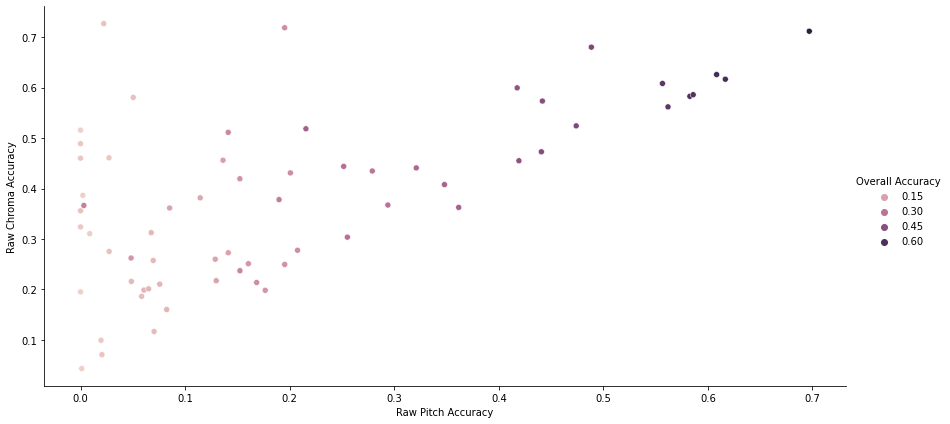
\includegraphics[width=\textwidth, height=5cm]{RESULTS}
\caption{\textit{Raw Chroma Accuracy} to \textit{Raw Pitch Accuracy} ratio}
\end{figure}

\begin{figure}[H]
\centering
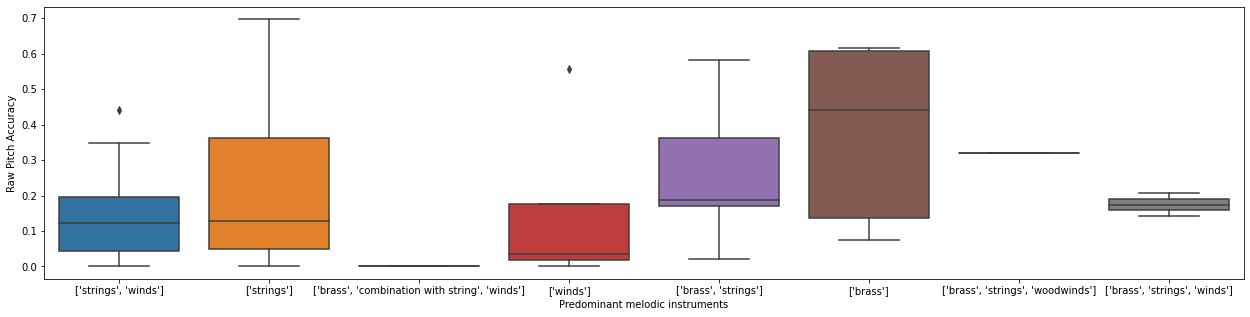
\includegraphics[width=\textwidth, height=5cm]{RAW PITCH ACCURACY BOX}
\caption{\textit{Raw Pitch Accuracy} to instrument family distribution}
\end{figure}

\begin{figure}[H]
\centering
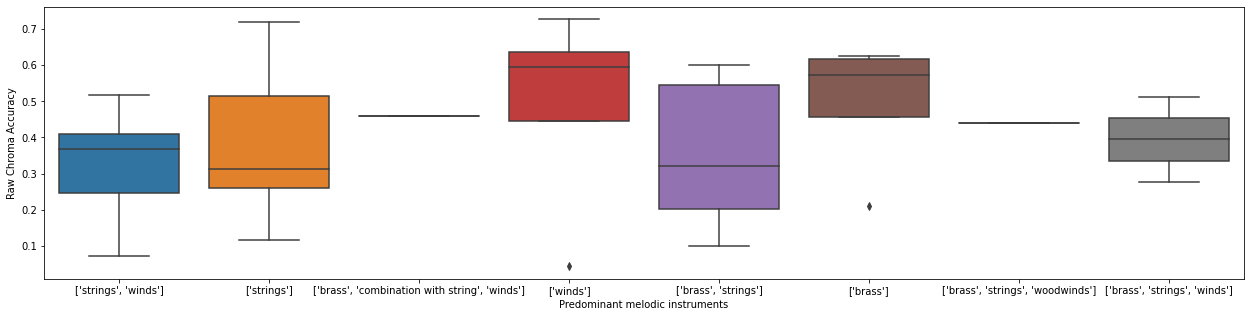
\includegraphics[width=\textwidth, height=5cm]{images/RAW CHROMA ACCURACY BOX}
\caption{\textit{Raw Chroma Accuracy} to instrument family distribution}
\end{figure}

\section{Discussion}
\subsection{Is this a "\textit{fair trial}" for \textit{Predominant Pitch Melodia Algorithm}?}
I think it is \textbf{not} and it is due to: 1) the "\textit{human nature}" of the recordings as well as the 2) inevitable subjective factor when choosing the excerpts melodic contours in the dataset.
\paragraph{Human error}Refers to something having been done that was "\textit{not intended by the actor; not desired by a set of rules or an external observer; or that led the task or system outside its acceptable limits}". This plays a big role in MIR evaluation, especially in the classical music domain.
\subparagraph{Performance}In contemporary production, when removing all the imperfections of slight pitch variance from track to track, we lose the subtle chorusing and thickening effect that happens. Perfectly in-tune tracks will be perceived as small and thin. That is why an orchestra plays beautifully "out of tune".
\subparagraph{Data annotation}Some inconsistencies and/or discrepancies might be found in the data annotation within the dataset. Subtle things such as chosen octave or melodic contour given the premise that the melody is “\textit{the single (monophonic) pitch sequence that a \textbf{listener might reproduce} if asked to whistle or hum a piece of polyphonic music}” as this have a huge subjective connotation and it is closely related to the individual cultural/musical background.

\subsection{About the data distribution: does it make sense from a analytical MIR perspective?}
It does as \textit{Raw Chroma Accuracy} is less sensitive than \textit{Raw Pitch Accuracy}. Energy detection around a pitch class will always lead the process of eventually detecting the specific pitch segment, but never the other way round. That is why the \textit{relplot} describes such clear lineal discrimination between axis.

\subsection{About the data distribution: does it make sense from a musicological perspective?}
The big picture of the \textit{scatter plot} does. Strings are well-suited to playing melody, as well as accompaniment, making them one of the most important instruments in the orchestra. A symphony orchestra is usually made up of around 10 first violins and 10 second violins, 10 violas, 8 cellos, and 6 double basses which generates a big chorus effect that translates into a "blurry" pitch sensation.

The brass is generally considered the loudest instrument in the modern orchestra. Along with woodwinds, the section is usually made between \textit{a2} and \textit{a4} which means between 2 and 4 which provides a lighter -not to mention nonexistent- chorus effect.

The only results that concern me are the \textit{Raw Pitch Accuracy} for the woodwinds. Given their characteristics and their high \textit{Raw Chroma Accuracy} results, the \textit{Raw Pitch Accuracy} results are significantly lower than what I had originally expected them to be.

\bibliographystyle{unsrtnat}
\bibliography{references}
\cite{rachel_bittner_2019_3527750}
\cite{bosch_j_2016_1289786}
\cite{colin_raffel_2014_1416528}
\cite{jordan_lenchitz_2021_5624645}
\cite{international_society_for_music_informat_2021_5776687}
\cite{roger_b_dannenberg_2001_1418263}
\cite{dmitry_bogdanov_2013_1415016}
\cite{j_salamon_2012_1289780}

\end{document}